\documentclass[12pt]{article}

\usepackage{amsmath, mathtools}
\usepackage{amsfonts}
\usepackage{amssymb}
\usepackage{graphicx}
\usepackage{colortbl}
\usepackage{xr}
\usepackage{hyperref}
\usepackage{longtable}
\usepackage{xfrac}
\usepackage{tabularx}
\usepackage{float}
\usepackage{siunitx}
\usepackage{booktabs}
\usepackage{caption}
\usepackage{pdflscape}
\usepackage{afterpage}

\usepackage[round]{natbib}

%\usepackage{refcheck}

\hypersetup{
	bookmarks=true,         % show bookmarks bar?
	colorlinks=true,       % false: boxed links; true: colored links
	linkcolor=red,          % color of internal links (change box color with linkbordercolor)
	citecolor=green,        % color of links to bibliography
	filecolor=magenta,      % color of file links
	urlcolor=cyan           % color of external links
}

%% Comments

\usepackage{color}

\newif\ifcomments\commentstrue

\ifcomments
\newcommand{\authornote}[3]{\textcolor{#1}{[#3 ---#2]}}
\newcommand{\todo}[1]{\textcolor{red}{[TODO: #1]}}
\else
\newcommand{\authornote}[3]{}
\newcommand{\todo}[1]{}
\fi

\newcommand{\wss}[1]{\authornote{blue}{SS}{#1}}
\newcommand{\an}[1]{\authornote{magenta}{Author}{#1}}


% For easy change of table widths
\newcommand{\colZwidth}{1.0\textwidth}
\newcommand{\colAwidth}{0.13\textwidth}
\newcommand{\colBwidth}{0.82\textwidth}
\newcommand{\colCwidth}{0.1\textwidth}
\newcommand{\colDwidth}{0.05\textwidth}
\newcommand{\colEwidth}{0.8\textwidth}
\newcommand{\colFwidth}{0.17\textwidth}
\newcommand{\colGwidth}{0.5\textwidth}
\newcommand{\colHwidth}{0.28\textwidth}

% Used so that cross-references have a meaningful prefix
\newcounter{defnum} %Definition Number
\newcommand{\dthedefnum}{GD\thedefnum}
\newcommand{\dref}[1]{GD\ref{#1}}
\newcounter{datadefnum} %Datadefinition Number
\newcommand{\ddthedatadefnum}{DD\thedatadefnum}
\newcommand{\ddref}[1]{DD\ref{#1}}
\newcounter{theorynum} %Theory Number
\newcommand{\tthetheorynum}{T\thetheorynum}
\newcommand{\tref}[1]{T\ref{#1}}
\newcounter{tablenum} %Table Number
\newcommand{\tbthetablenum}{T\thetablenum}
\newcommand{\tbref}[1]{TB\ref{#1}}
\newcounter{assumpnum} %Assumption Number
\newcommand{\atheassumpnum}{P\theassumpnum}
\newcommand{\aref}[1]{A\ref{#1}}
\newcounter{goalnum} %Goal Number
\newcommand{\gthegoalnum}{P\thegoalnum}
\newcommand{\gsref}[1]{GS\ref{#1}}
\newcounter{instnum} %Instance Number
\newcommand{\itheinstnum}{IM\theinstnum}
\newcommand{\iref}[1]{IM\ref{#1}}
\newcounter{reqnum} %Requirement Number
\newcommand{\rthereqnum}{P\thereqnum}
\newcommand{\rref}[1]{R\ref{#1}}
\newcounter{lcnum} %Likely change number
\newcommand{\lthelcnum}{LC\thelcnum}
\newcommand{\lcref}[1]{LC\ref{#1}}

\newcommand{\progname}{Breaking Effect} % PUT YOUR PROGRAM NAME HERE

\usepackage{fullpage}

\begin{document}
	
	\title{Breaking Effect} 
	\author{Xiaoye Ma, max58@mcmaster.ca}
	\date{\today}
	
	\maketitle
	
	~\newpage
	
	\pagenumbering{roman}
	
	\section{Revision History}
	
	\begin{tabularx}{\textwidth}{p{3cm}p{2cm}X}
		\toprule {\bf Date} & {\bf Version} & {\bf Notes}\\
		\midrule
		2017-10-01 & 1.0 & New document\\
		\bottomrule
	\end{tabularx}
	
	~\newpage
	
	\section{Reference Material}
	
	This section records information for easy reference.
	
	\subsection{Table of Units}
	
	Throughout this document SI (Syst\`{e}me International d'Unit\'{e}s) is employed
	as the unit system.  In addition to the basic units, several derived units are
	used as described below.  For each unit, the symbol is given followed by a
	description of the unit and the SI name.
	~\newline
	
	\renewcommand{\arraystretch}{1.2}
	%\begin{table}[ht]
	\noindent \begin{tabular}{l l l} 
		\toprule		
		\textbf{symbol} & \textbf{unit} & \textbf{SI}\\
		\midrule 
		\si{\metre} & length & metre\\
		\si{\kilogram} & mass	& kilogram\\
		\si{\second} & time & second\\
		\si{\joule} & energy & Joule\\
		\bottomrule
	\end{tabular}
	%	\caption{Provide a caption}
	%\end{table}
	
	\subsection{Table of Symbols}
	
	The table that follows summarizes the symbols used in this document along with
	their units.  The choice of symbols was made to be consistent with the heat
	transfer literature and with existing documentation for solar water heating
	systems.  The symbols are listed in alphabetical order.
	
	\renewcommand{\arraystretch}{1.2}
	%\noindent \begin{tabularx}{1.0\textwidth}{l l X}
	\noindent \begin{longtable*}{l l p{12cm}} \toprule
		\textbf{symbol} & \textbf{unit} & \textbf{description}\\
		\midrule 
		$S$ & unit of length & displacement
		\\
		$t$ & \si[per-mode=symbol] s & the time in seconds since the start of the game
		\\  
		$v_{0}$ & \si[per-mode=symbol] m/s & initial speed
		\\ 
		$a$ & $m/s^2$ & acceleration
		\\
		$g$ & $m/s^2$ & gravity acceleration
		\\
		$\Delta E_{k}$ & J & variation of kinetic energy
		\\
		$\Delta E_{p}$ & J & variation of potential energy
		\\
		$W_{f}$ & $J$ & work done by kinetic friction
		\\
		$x_{n}$ & $m$ & x coordinates of gravity center of piece $n$, $n \in \mathbb{N}$, which represents just one piece. \wss{Explain the
			meaning of $n$?  Also, you should format it like a mathematical variable ($n$,
			not n).}\an{Add explanation for $n$ and format it as a mathematical variable.}
		\\
		$y_{n}$ & $m$ & y coordinates of gravity center of piece n
		\\
		$z_{n}$ & $m$ & z coordinates of gravity center of piece n
		\\
		$\theta_{1}$ & degree & angle between initial speed and horizontal
		\\
		$\theta_{2}$ & degree & angle between
		x axiom and projection on horizontal of initial speed
		\\
		$S_{x}$ & $m$ & displacement on direction of x axiom
		\\
		$S_{y}$ & $m$ & displacement on direction of y axiom
		\\
		$S_{z}$ & $m$ & displacement on direction of z axiom
		\\
		$\mu_k$ &  & coefficient of friction
		\\
		\bottomrule
	\end{longtable*}
	
	\subsection{Abbreviations and Acronyms}
	
	\renewcommand{\arraystretch}{1.2}
	\begin{tabular}{l l} 
		\toprule		
		\textbf{symbol} & \textbf{description}\\
		\midrule 
		A & Assumption\\
		DD & Data Definition\\
		GD & General Definition\\
		GS & Goal Statement\\
		IM & Instance Model\\
		LC & Likely Change\\
		PS & Physical System Description\\
		R & Requirement\\
		SRS & Software Requirements Specification\\
		\progname{} & Breaking Effect\\
		T & Theoretical Model\\
		\bottomrule
	\end{tabular}\\
	
	\newpage
	
	\tableofcontents
	
	~\newpage
	
	\pagenumbering{arabic}
	
	\section{Introduction}
	
	Breaking effect presents how the pieces of an object move after it separates into parts with suddenness or violence. \an{Add explanation for BE here}
	
	Because of the development of video games industrial and hardware such as CPU
	and GPU, there is a higher demand for high level experience in game
	visualization. Breaking effect plays a more important role in the visualization
	level of large scale video games. \wss{Tell the reader what the breaking effect
		is.}  This project simulates the process of 3D objects’ destruction.
	
	The following section provides an overview of the Software Requirements Specification (SRS) for a breaking effect program. The developed program will be referred to as Breaking Effect (BE). This section explains the purpose of this document, the scope of the system, the characteristics of the intended readers and the organization of the document.
	
	\wss{The text is better for version control, and for reading in other editors,
		if you use a hard-wrap at 80 characters}
	
	\subsection{Purpose of Document}
	
	The main purpose of this document is to describe the modeling of breaking effect. The goals and theoretical models used in the breaking effect code are provided, with an emphasis on explicitly identifying assumptions and unambiguous definitions. 
	
	\subsection{Scope of Requirements} 
	
	The scope of the requirements is limited to breaking effect of a single 3D object applied by force. Interact force between objects and collision among several objects are not in the scope. Given the appropriate inputs, the code for BE is intended to calculate pieces motion and display the process of target 3D object breaking in vision. The project is implemented in a game engine. 3-D objects and piece generation function are provided by platform. 
	
	\subsection{Characteristics of Intended Reader} 
	
	Reviewers of this documentation should have a strong knowledge in physics motion theory and an understanding of differential equations. A third year Physics course on this topic in high school is recommended.  \wss{For the
		characteristics of intended reader try to be more specific about the
		education.  What degree?  What course areas?  What level?} \an{Add specific course and level}
	
	\subsection{Organization of Document}
	
	The organization of this document follows the template for an SRS for scientific
	computing software proposed by \citet{SmithAndLai2005, SmithEtAl2007}. \an{Copy the format from original template.} The
	presentation follows the standard pattern of presenting goals, theories,
	definitions, and assumptions. \wss{You should use BibTeX for this.  The original
		template showed you how to do this.  If you have questions about how to use
		BibTeX, please ask your classmates, or me.}
	
	\section{General System Description}
	
	This section identifies the interfaces between the system and its environment,
	describes the user characteristics and lists the system constraints.
	
	\subsection{System Context}
	
	\begin{figure}
		\centering
		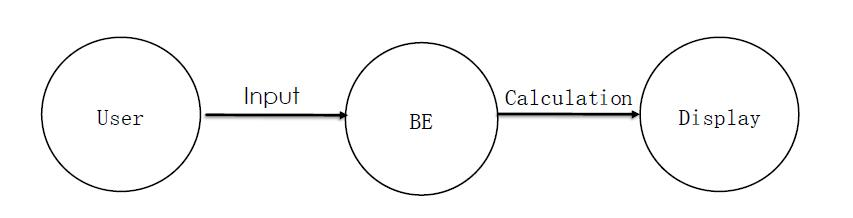
\includegraphics[width=0.7\linewidth]{./f18}
		\caption{}
		\label{fig:f18}
	\end{figure}
	
	\begin{itemize}
		\item User Responsibilities:
		\begin{itemize}
			\item Provide inputs and make sure they are in an appropriate range including position of target object, initial momentum, coefficient of friction on the ground. \wss{Try to
				be more specific about what inputs the user provides.  Determining whether
				inputs are in the appropriate range seems like something your program could
				easily test.}\an{Yes ! Make this more specific by listing necessary inputs.}
		\end{itemize}
		\item \progname{} Responsibilities:
		\begin{itemize}
			\item Detect data type mismatch, such as a string of characters instead of a
			floating point number
			\item Determine if the inputs satisfy the required physical and software constraints as shown in \ref{sec_DataConstraints}.​ \wss{Is the appropriate range (from the user responsibilities
				above) included in the constraints?}\an{Refer to data constraints section.}
			\item Calculate the required outputs
		\end{itemize}
	\end{itemize}
	
	\subsection{User Characteristics} \label{SecUserCharacteristics}
	
	The end user of \progname{} should have a basic knowledge of Physics and Dimensional geometry as well as experience of using Unity3D. A background of high school level Physics and Dimensional geometry course are recommended. \wss{Please be more specific on the users education background and level.}\an{Add specific course and level.}
	
	\subsection{System Constraints}
	
	This project is implemented in Unity3D because it relies on 3D models and existing function for object cutting. Users have to use Break effect in Unity3D project. The algorithm can be implemented in other physics engines but for practical reasons they will not be considered in this project.  \wss{I think you have to include Unity as a
		system constraint, or remove the mention of it elsewhere in the document.  You
		have obviously (for practical reasons) decided that you are going to use
		Unity.  You should explicitly inform the user of this.  I also suggest that
		you mention that there are other options for physics engines, but for
		practical reasons they will not be considered in this project.}\an{Include Unity3D as a system constraint and provide more information for users.}
	
	\section{Specific System Description}
	
	This section first presents the problem description, which gives a high-level
	view of the problem to be solved.  This is followed by the solution characteristics
	specification, which presents the assumptions, theories, definitions and finally
	the instance models. 
	
	\subsection{Problem Description} \label{Sec_pd}
	
	This project tries to implement running time breaking effect in codes for 3-D models in unity3D without help from any similar plug-in. Including different shapes 3-D objects breaking based on physics and pieces interacting with the momentum provided by the breaking force. The breaking effect program simulates 3-D objects’ destruction process in vision by implementing scientific computing functions. This project concentrates on calculation while HCI or GUI are not important parts. Applied force is decided in codes in advance as input and trace of motion is the output after calculation.
	
	\subsubsection{Terminology and  Definitions}
	
	This subsection provides a list of terms that are used in the subsequent
	sections and their meaning, with the purpose of reducing ambiguity and making it
	easier to correctly understand the requirements:
	
	\begin{itemize}
		
		\item Focus point: The location where explosion happens \wss{spell check!}\an{Fixed. Sorry for the mistake !}
		\item initial momentum level: Initial momentum of pieces  
		
	\end{itemize}
	
	\subsubsection{Physical System Description}
	
	The physical system of \progname{} includes visual terrain \wss{spell check!}\an{Fixed. Sorry for the mistake !} and a target 3-D object which will break into pieces.
	
	% \begin{figure}[h!]
	% \begin{center}
	% %\rotatebox{-90}
	% {
	%  \includegraphics[width=0.5\textwidth]{<FigureName>}
	% }
	% \caption{\label{<Label>} <Caption>}
	% \end{center}
	% \end{figure}
	
	\subsubsection{Goal Statements}
	
	\noindent Given the target object, coefficient of friction, focus point and initial momentum level, the goal statements are:
	
	\begin{itemize}
		
		\item[GS\refstepcounter{goalnum}\thegoalnum \label{G_speed}:] Calculate initial speed of each piece.​
		
		\item[GS\refstepcounter{goalnum}\thegoalnum \label{G_motion}:] Calculate trace of motion for each piece.
		
	\end{itemize}
	
	\subsection{Solution Characteristics Specification}
	
	The instance models that govern \progname{} are presented in
	Subsection~\ref{sec_instance}.  The information to understand the meaning of the
	instance models and their derivation is also presented, so that the instance
	models can be verified.
	
	\subsubsection{Assumptions}
	
	This section simplifies the original problem and helps in developing the
	theoretical model by filling in the missing information for the physical
	system. The numbers given in the square brackets refer to the theoretical model
	[T], general definition [GD], data definition [DD], instance model [IM], or
	likely change [LC], in which the respective assumption is used.
	
	\begin{itemize}
		
		\item[A\refstepcounter{assumpnum}\theassumpnum \label{A_mechanical}:]
		The forms of energy that are relevant for this problem are kinetic energy and potential energy. Thermal energy is considered on the ground but it is assumed to be negligible in the air. All other forms of energy are negligible. \wss{but you have friction?  Work will be
			done that eventually uses up the initial energy.}\an{Yes, I do consider kinetic friction on the ground and only air friction is ignored. I modify A1 and A2 to make them more specific. Sorry for the confusion !}
		
		\item[A\refstepcounter{assumpnum}\theassumpnum \label{A_airFriction}:]
		Air friction will be ignored while kinetic friction is considered on the ground and it is assumed to be constant.
		
		\item[A\refstepcounter{assumpnum}\theassumpnum \label{A_powder}:]
		Powders and airborne \wss{spell check!} \an{Fixed, sorry for the mistake !}dust will not be considered. Because they both have random shapes, motions and they are seriously influenced by air friction. Powders are considered as very tiny size pieces that are generated in explosion.
		\wss{missing period.} \wss{What makes a piece powder?  How is powder defined?}\an{Add explanation for powder and airborne dust.}
		
		\item[A\refstepcounter{assumpnum}\theassumpnum \label{A_initialPE}:]
	Before explosion, the kinetic energy and potential energy of target object are zero. Target object cannot be a moving object. An initial momentum will be assigned to each piece after explosion happens. \wss{You
			say in your goal statement that there is an initial momentum.  If the kinetic
			energy is zero, then the momentum will always be }\an{There is some misunderstanding in this assumption. The initial energy here represents the energy before explosion. And initial momentum in GS refers to the energy after explosion happens. So they are totally different status because of different periods. I modify the expression to make it clearer. Sorry for the confusion !}
		
		\item[A\refstepcounter{assumpnum}\theassumpnum \label{A_ground}:]
		The same coefficient of friction everywhere on flat ground.​
		
		\item[A\refstepcounter{assumpnum}\theassumpnum \label{A_piece}:]
		Pieces are not decomposable. 
		
		\item[A\refstepcounter{assumpnum}\theassumpnum \label{A_collision}:]
		Collision between pieces will not be considered. 
		
	\end{itemize}
	
	\subsubsection{Theoretical Models}\label{sec_theoretical}
	
	This section focuses on the general equations and laws that \progname{} is based
	on. 
	
	~\newline
	
	\noindent
	\begin{minipage}{\textwidth}
		\renewcommand*{\arraystretch}{1.5}
		\begin{tabular}{| p{\colAwidth} | p{\colBwidth}|}
			\hline
			\rowcolor[gray]{0.9}
			Number& T\refstepcounter{theorynum}\thetheorynum \label{T_CME}\\
			\hline
			Label&\bf Conservation of mechanical energy\\
			\hline
			Equation&  $E_{mech}=E_{k}+E_{p}$\\
			\hline
			
			Description & 
			The total mechanical energy (defined as the sum of its potential
			and kinetic energies) of a particle being acted on
			by only conservative forces is constant. The
			potential energy, $E_{p}$, depends on the position
			of an object subjected to a conservative
			force. The kinetic energy, $E_{k}$, depends on the
			speed of an object and is the ability of a moving
			object to do work on other objects when it
			collides with them.Assumption \ref{A_airFriction} is necessary for this equation to be true when pieces move in the air. This TM only works for motion in the air. After explosion happens, pieces do parabolic movement on vertical direction in which acceleration is always $g$, and do uniform motion on horizontal direction in the air.  \wss{What about the work done
				by nonconservative forces, like friction?  This should be part of
				your conservation of energy.  The equation you
				have written is only true in the case where the
				work done by nonconservative forces is zero.  You
				should also reference the assumptions that are
				necessary for your theoretical model to apply.}\an{When pieces move in the air, nonconservative forces are ignored so that only energy are considered. When pieces move on the ground, I do consider kinetic friction. This TM only works for motion in the air. While T2 below is used for motion on the ground. I modify the description to make it clearer. }\\
			\hline
			Source &
			\url{http://www.nuclear-power.net/laws-of-conservation/law-of-conservation-of-energy/conservation-of-mechanical-energy/}\\
			% The above web link should be replaced with a proper citation to a publication
			\hline
			Ref.\ By & \iref{IM_DIA}\\
			\hline
		\end{tabular}
	\end{minipage}\\
	
	~\newline
	
	\noindent
	\begin{minipage}{\textwidth}
		\renewcommand*{\arraystretch}{1.5}
		\begin{tabular}{| p{\colAwidth} | p{\colBwidth}|}
			\hline
			\rowcolor[gray]{0.9}
			Number& T\refstepcounter{theorynum}\thetheorynum \label{T_WKF}\\
			\hline
			Label&\bf Work done by kinetic friction\\
			\hline
			Equation&  $\Delta E_{k}=W_{f}$\\
			\hline
			
			Description & 
			Kinetic energy loses due to kinetic energy. $W_{f}$ is work done by kinetic friction. As a result, kinetic energy transform to internal energy.When piece move on the ground, they do constant decelerated motion and acceleration is constant and negative because of constant kinetic friction on the ground.\\
			\hline
			Source &
			\url{http://teacher.pas.rochester.edu/phy121/lecturenotes/Chapter07/Chapter7.html}\\
			% The above web link should be replaced with a proper citation to a publication
			\hline
			Ref.\ By & \iref{IM_DOG}\\
			\hline
		\end{tabular}
	\end{minipage}\\
	
	~\newline
	
	\subsubsection{General Definitions}\label{sec_gendef}
	
	There is no general definition for current problem.
	
	\subsubsection{Data Definitions}\label{sec_datadef}
	
	This section collects and defines all the data needed to build the instance
	models. The dimension of each quantity is also given. 
	
	~\newline
	
	\noindent
	\begin{minipage}{\textwidth}
		\renewcommand*{\arraystretch}{1.5}
		\begin{tabular}{| p{\colAwidth} | p{\colBwidth}|}
			\hline
			\rowcolor[gray]{0.9}
			Number& DD\refstepcounter{datadefnum}\thedatadefnum \label{DD_UAM}\\
			\hline
			Label& \bf Displacement in uniformly accelerated/decelerated motion\\
			\hline
			Symbol &$S$\\
			\hline
			% Units& $Mt^{-3}$\\
			% \hline
			SI Units & M\\
			\hline
			Equation&$S= v_{0}t+\frac{1}{2}at^{2}$\\
			\hline
			Description & 
			The above equation gives us the distance traveled without
			having to know the final velocity of the object. Where $t$ is
			time duration and $v_{0}$ is initial speed. Acceleration $a$ is
			defined as the rate of change of velocity with respect to time,
			in a given direction. This would mean that if an object has an
			acceleration of 1 $m/s^{2}$ it will increase its velocity (in a given direction) 1 $m/s$ every second that it accelerates. This
			equation is tenable under \aref{A_mechanical},
			\aref{A_airFriction} and \aref{A_ground} in this project.
			\wss{This equation only applies for constant acceleration.  As
				the object loses energy the acceleration will decrease.  None of
				your assumptions mention assuming constant acceleration.  The
				equation you are using comes from kinematics, where you don't
				need to worry about forces.  I think you do have to worry about
				forces, which moves it to the area of kinetics.}\an{Sorry that I made it confused here. Actually I believe it is a misunderstanding due to my unspecific expression. I do consider deceleration because of work done gravity force when pieces move in the air and work done by friction when pieces move on the ground. I add decelerated motion in label above and modify assumption 2 to consider kinetic friction on the ground as constant force. And since gravity and friction are considered as constant force, acceleration are constant positive and negative respectively.}
			\\
			\hline
			Sources&~\url{http://ibphysicsstuff.wikidot.com/uniformaccmotion}  \\
			\hline
			Ref.\ By & \iref{IM_DIA},\iref{IM_DOG}\\
			\hline
		\end{tabular}
	\end{minipage}\\
	
	\subsubsection*{Derivation of how to derive the equation from relationship of position, velocity and acceleration}
	
	~\newline
	We assume $v_{0}$ is initial velocity and $v_{t}$ is the final velocity. 
	
	~\newline
	Then we have:
	$v_{t}=v_{0}+at$
	
	~\newline
	We can get average velocity $v_{a}$
	~\newline
	$v_{a}=\frac{v_{0}+v_{t}}{2}$
	
	~\newline
	So we can get displacement
	
	~\newline 
	$S=v_{a}t=\frac{v_{0}+v_{t}}{2}t$
	
	~\newline
	$S=\frac{v_{0}+v_{0}+at}{2}t=v_{0}t+\frac{1}{2}at^{2}$
	
	
	~\newline
	
	\noindent
	\begin{minipage}{\textwidth}
		\renewcommand*{\arraystretch}{1.5}
		\begin{tabular}{| p{\colAwidth} | p{\colBwidth}|}
			\hline
			\rowcolor[gray]{0.9}
			Number& DD\refstepcounter{datadefnum}\thedatadefnum \label{DD_Fk}\\
			\hline
			Label& \bf Kinetic friction\\
			\hline
			Symbol &$F_{k}$\\
			\hline
			% Units& $Mt^{-3}$\\
			% \hline
			SI Units & N\\
			\hline
			Equation&$F_{k}=\mu_{k}F_{n}=\mu_{k}mg$\\
			\hline
			Description & 
			Kinetic friction $F_{k}$ is a force that acts between moving
			surfaces. An object that is being moved over a
			surface will experience a force in the opposite
			direction as its movement. The magnitude of the
			force depends on the coefficient of kinetic
			friction between the two kinds of material. Every
			combination is different. The coefficient of
			kinetic friction is assigned the Greek letter ``mu''
			$\mu$, with a subscript ``k''.  \wss{Use ``quote'' to
				get correct quotation marks} The force of kinetic
			friction is $\mu_{k}$ times the normal force on an
			object, and is expressed in units of Newtons (N).
			In this project, $F_{n}$ equals to
			$mg$. \wss{gravity is an acceleration, not a
				force.  Your force is $mg$, where $m$ is the mass
				of the object.  Do you know the mass of the objects?}\an{Yeah actually I know force is $mg$, $g$ is acceleration. However I am not sure if gravity in English means gravitational force
				Maybe the confusion here is because I misuse the word. }
			\\
			\hline
			Sources&~\url{http://www.softschools.com/formulas/physics/kinetic_friction_formula/92/}  \\
			\hline
			Ref.\ By & \iref{IM_DOG}\\
			\hline
		\end{tabular}
	\end{minipage}\\
	
	\subsubsection{Instance Models} \label{sec_instance}    
	
	This section transforms the problem defined in Section~\ref{Sec_pd} into 
	one which is expressed in mathematical terms. It uses concrete symbols defined 
	in Section~\ref{sec_datadef} to replace the abstract symbols in the models 
	identified in Sections~\ref{sec_theoretical} and~\ref{sec_gendef}.
	
	The goals \gsref{G_speed} and \gsref{G_motion} are solved by \iref{IM_angle} to \iref{IM_DOG}.
	Piece generation is done by calling cutting function in game engine.   
	
	~\newline
	
	%Instance Model 1
	
	\noindent
	\begin{minipage}{\textwidth}
		\renewcommand*{\arraystretch}{1.5}
		\begin{tabular}{| p{\colAwidth} | p{\colBwidth}|}
			\hline
			\rowcolor[gray]{0.9}
			Number& IM\refstepcounter{instnum}\theinstnum \label{IM_angle}\\
			\hline
			Label& \bf Find the angle between $v_{0}$ and horizontal. Find the angle between x axiom and projection on horizontal of initial speed \\
			\hline
			Input&$x_{n}$,$y_{n}$,$z_{n}$\\
			\hline
			Output&$\theta_{1}=arctan \frac{|z_{n}|}{\sqrt{x_{n}^2+y_{n}^2}}$\\
			&$\theta_{2}=arctan \frac{y_{n}}{x_{n}}$\\
			\hline
			Description&$x_{n}$ is x coordinates of gravity center of piece n.\\
			&$y_{n}$ is y coordinates of gravity center of piece n.\\
			&$z_{n}$ is z coordinates of gravity center of piece n.\\
			\hline
			Sources&~\ \ \\
			\hline
			Ref.\ By & \iref{IM_DIA}\\
			\hline
		\end{tabular}
	\end{minipage}\\
	
	~\newline
	
	\noindent
	\begin{minipage}{\textwidth}
		\renewcommand*{\arraystretch}{1.5}
		\begin{tabular}{| p{\colAwidth} | p{\colBwidth}|}
			\hline
			\rowcolor[gray]{0.9}
			Number& IM\refstepcounter{instnum}\theinstnum \label{IM_DIA}\\
			\hline
			Label& \bf Uniformly accelerated motion to find displacement in the air\\
			\hline
			Input&$v_{0}$,$\theta_{1}$ from IM1,$\theta_{2}$ from IM1,$t$,$g$\\
			\hline
			Output&$S_{x}=v_{0}\cdot cos\theta _{1}\cdot cos\theta _{2}\cdot t$\\
			&$S_{y}=v_{0}\cdot cos\theta _{1}\cdot sin\theta _{2}\cdot t$,\\
			&$S_{z}=v_{0}\cdot sin\theta _{1}\cdot t-\frac{1}{2}gt^{2}$\\
			\hline
			Description&$v_{0}$ is the initial speed.\\
			&$t$ is time from beginning.\\
			&$\theta _{1}$ is the angle between $v_{0}$ and horizontal.\\
			&$\theta _{2}$ is the angle between x axiom and projection on horizontal of initial speed.\\
			& The above equation applies as long as the piece moving in the air.
			\\
			\hline
			Sources&~\ \ \\
			\hline
			Ref.\ By & \\
			\hline
		\end{tabular}
	\end{minipage}\\
	
	~\newline
	
	\noindent
	\begin{minipage}{\textwidth}
		\renewcommand*{\arraystretch}{1.5}
		\begin{tabular}{| p{\colAwidth} | p{\colBwidth}|}
			\hline
			\rowcolor[gray]{0.9}
			Number& IM\refstepcounter{instnum}\theinstnum \label{IM_DOG}\\
			\hline
			Label& \bf Uniformly accelerated motion to find displacement on the ground\\
			\hline
			Input&$v_{0}$,$\theta_{1}$,$\theta_{2}$,$t$,$g$,$\mu_{k}$\\
			\hline
			Output&$a=\mu_{k}g$\\
			&$S_{x}=v_{0}\cdot cos\theta _{1}\cdot cos\theta _{2}\cdot t-\frac{1}{2}at^{2}$\\
			&$S_{y}=v_{0}\cdot cos\theta _{1}\cdot sin\theta _{2}\cdot t-\frac{1}{2}at^{2}$,\\
			\hline
			Description&$v_{0}$ is the initial speed.\\
			&$t$ is time from beginning.\\
			&$\theta _{1}$ is the angle between $v_{0}$ and horizontal.\\
			&$\theta _{2}$ is the angle between x axiom and projection on horizontal of initial speed.\\
			&$\mu_{k}$ is the Coefficient of friction.\\
			& The above equation applies as long as the piece moving on the ground.
			\\
			\hline
			Sources&~\ \ \\
			\hline
			Ref.\ By & \\
			\hline
		\end{tabular}
	\end{minipage}\\
	
	%~\newline
	
	\subsubsection*{Derivation of how to get angle between $v_{0}$ and horizontal}
	
	We have initial location (X,Y,Z) of target object, and location $(x_{n},y_{n},z_{n})$ for piece n, then we can calculate the angle between $v_{0}$ and horizontal by:
	~\newline
	\\
	$tan\theta_{1}=\frac{|z_{n}-Z|}{\sqrt{(x_{n}-X)^{2}+(y_{n}-Y)^{2}}}$
	~\newline
	\\
	If location of target object is (0,0,0), then we have:
	~\newline
	\\
	$tan\theta_{1}=\frac{|z_{n}|}{\sqrt{x_{n}^{2}+y_{n}^{2}}}$
	~\newline
	\\
	$\theta_{1}=arctan \frac{|z_{n}|}{\sqrt{x_{n}^2+y_{n}^2}}$
	~\newline
	\\
	
	\wss{You really need to work on the physics in your project. You might
		understand the physics better when you proceed to the next steps.  For
		instance, you will learn about the problems with applying DD1 - your particles
		would never stop, they would just keep accelerating.  For your project faking
		a rational design process should be very helpful.}
	\an{Sorry for the confusion here ! Actually when pieces move on the ground, the acceleration $a$ in DD1 is a negative number because I do consider friction on the ground. So that particles do constant decelerated motion and will actually stop eventually. In fact, after explosion happens, pieces do parabolic movement on vertical direction in which acceleration is always $g$, and do uniform motion on horizontal direction in the air. When piece move on the ground, they do constant decelerated motion and acceleration is constant and negative because of constant kinetic friction on the ground. I add more expression in my TM to make my models clearer.}
	\wss{You don't say how the object will be broken into pieces.  You have this
		goal, but as far as I can tell, you never return to it.  You should add goals
		to your traceability matrix, so that you would see this omission.}
	\an{I prefer to use existing function provided by Unity3D because how to split the object into pieces is not emphasis. I can specify this in system constrain and delete object cutting in GS1.}
	\subsubsection{Data Constraints} \label{sec_DataConstraints}    
	
	Tables~\ref{TblInputVar} and \ref{TblOutputVar} show the data constraints on the
	input and output variables, respectively.  The column for physical constraints gives
	the physical limitations on the range of values that can be taken by the
	variable.  The column for software constraints restricts the range of inputs to
	reasonable values.  The constraints are conservative, to give the user of the
	model the flexibility to experiment with unusual situations.  The column of
	typical values is intended to provide a feel for a common scenario.  The
	uncertainty column provides an estimate of the confidence with which the
	physical quantities can be measured.  This information would be part of the
	input if one were performing an uncertainty quantification exercise.
	
	The specification parameters in Table~\ref{TblInputVar} are listed in
	Table~\ref{TblSpecParams}.
	
	\begin{table}[!h]
		\caption{Input Variables} \label{TblInputVar}
		\renewcommand{\arraystretch}{1.2}
		\noindent \begin{longtable*}{l l l l c} 
			\toprule
			\textbf{Var} & \textbf{Physical Constraints} & \textbf{Software Constraints} &
			\textbf{Typical Value} & \textbf{Uncertainty}\\
			\midrule 
			$X$ &  & $L_{\text{min}} \leq X \leq L_{\text{max}}$ & 0 & 10\%
			\\
			$Y$ &  & $L_{\text{min}} \leq Y \leq L_{\text{max}}$ & 0 & 10\%
			\\
			$Z$ &  & $0$ & 0 & 0\%
			\\
			$x_{n}$ &  & $L_{\text{min}} \leq x_{n} \leq L_{\text{max}}$ & 0 & 10\%
			\\
			$y_{n}$ &  & $L_{\text{min}} \leq y_{n} \leq L_{\text{max}}$ & 0 & 10\%
			\\
			$z_{n}$ &  & $L_{\text{min}} \leq z_{n} \leq L_{\text{max}}$ & 0 & 10\%
			\\
			$v_{0}$ & $v_{0} > 0$ & $v_{\text{min}} \leq v_{0} \leq v_{\text{max}}$ & 20 m/s & 10\%
			\\
			$\mu_{k}$ & $\mu_{k} > 0$ & $\mu_{\text{min}} \leq \mu_{k} \leq \mu_{\text{max}}$ & 0.05 & 10\%
			\\
			$E$ &  & $E_{\text{min}} \leq E \leq E_{\text{max}}$ & 5 & 10\%
			\\
			\bottomrule
		\end{longtable*}
	\end{table}
	
	\noindent 
	
	\begin{table}[!h]
		\caption{Specification Parameter Values} \label{TblSpecParams}
		\renewcommand{\arraystretch}{1.2}
		\noindent \begin{longtable*}{l l} 
			\toprule
			\textbf{Var} & \textbf{Value} \\
			\midrule 
			$v_\text{min}$ & 10 m/s\\
			$v_\text{max}$ & 100 m/s\\
			$L_\text{min}$ & -1000\\
			$L_\text{max}$ & 1000\\
			$\mu_\text{min}$ & 0\\
			$\mu_\text{max}$ & 1\\
			\bottomrule
		\end{longtable*}
	\end{table}
	
	\begin{table}[!h]
		\caption{Output Variables} \label{TblOutputVar}
		\renewcommand{\arraystretch}{1.2}
		\noindent \begin{longtable*}{l l} 
			\toprule
			\textbf{Var} & \textbf{Physical Constraints} \\
			\midrule 
			$S_{x}$ & $S_{x} \geq 0$
			\\
			$S_{y}$ & $S_{y} \geq 0$
			\\
			$S_{z}$ & $S_{z} \geq 0$
			\\
			\bottomrule
		\end{longtable*}
	\end{table}
	
	\subsubsection{Properties of a Correct Solution} \label{sec_CorrectSolution}
	
	\noindent
	A correct solution must exhibit the principle of motion as well as conservation of energy.
	
	\section{Requirements}
	
	This section provides the functional requirements, the business tasks that the
	software is expected to complete, and the nonfunctional requirements, the
	qualities that the software is expected to exhibit.
	
	\subsection{Functional Requirements}
	
	\noindent \begin{itemize}
		
		\item[R\refstepcounter{reqnum}\thereqnum \label{R_Inputs}:] 
		Input the following quantities, which define the target object
		and initial conditions:
		\noindent \begin{longtable*}{l l l} 
			\toprule
			\textbf{symbol} & \textbf{unit} & \textbf{description}\\
			\midrule 
			$X$ & & x coordinates of target object
			\\
			$Y$ & & y coordinates of target object
			\\
			$Z$ & & z coordinates of target object
			\\
			$E$ & & Initial momentum level
			\\
			$\mu_{k}$ & & Coefficient of friction everywhere on flat ground
			\\
			\bottomrule
		\end{longtable*}
		
		~\newpage
		
		\item[R\refstepcounter{reqnum}\thereqnum \label{R_InitialSpeed}:] Use inputs in R1 to find initial speed $v_{0}$, as follows:
		
		$v_{0}=E \cdot 10$
		
		\item[R\refstepcounter{reqnum}\thereqnum \label{R_VerifyOutput}:] Verify that the inputs satisfy the required physical constraints shown in Table 1.
		
		\item[R\refstepcounter{reqnum}\thereqnum \label{R_Piece}:] Generate pieces by calling cutting function in game engine. Then get gravity center of each piece.
		
		\item[R\refstepcounter{reqnum}\thereqnum \label{R_Calculate}:]
		Calculate the angle between $v_{0}$ and horizontal($\theta _{1}$). Calculate the angle between x axiom and projection on horizontal of initial speed($\theta _{2}$) by IM\ref{IM_angle}. 
		
		\item[R\refstepcounter{reqnum}\thereqnum \label{R_Output1}:] 
		Calculate and output trace of motion for each piece in the air($S_{x},S_{y},S_{z}$) by IM\ref{IM_DIA}.
		
		\item[R\refstepcounter{reqnum}\thereqnum \label{R_Output2}:] 
		Calculate and output trace of motion for each piece on the ground($S_{x},S_{y},S_{z}$) by IM\ref{IM_DOG}.
		
	\end{itemize}
	
	\wss{Functional requirements should reference the instance models.}
	\an{Reference instance models.}
	\subsection{Nonfunctional Requirements}
	
	Performance is influenced by amount of pieces, capability of GPU and CPU. Other nonfunctional requirements are correctness and reusability.
	
	\wss{More information on the NFRs would improve this document.}
	\an{Haven't come up with other good points for NFRs. Will keep thinking ! }
	\section{Likely Changes}    
	
	\noindent \begin{itemize}
		
		\item[LC\refstepcounter{lcnum}\thelcnum\label{LC_SOP}:] \aref{A_ground} - In real situation, users may have kinds of terrians and textures. As a result, coefficient of friction needs to be changed correspondingly. 
		
	\end{itemize}
	
	\section{Traceability Matrices and Graphs}
	
	The purpose of the traceability matrices is to provide easy references on what
	has to be additionally modified if a certain component is changed.  Every time a
	component is changed, the items in the column of that component that are marked
	with an ``X'' may have to be modified as well.  Table~\ref{Table:trace} shows the
	dependencies of theoretical models, general definitions, data definitions, and
	instance models with each other. Table~\ref{Table:R_trace} shows the
	dependencies of instance models, requirements, and data constraints on each
	other. Table~\ref{Table:A_trace} shows the dependencies of theoretical models,
	general definitions, data definitions, instance models, and likely changes on
	the assumptions.
	
	
	\afterpage{
		\begin{landscape}
			\begin{table}[h!]
				\centering
				\begin{tabular}{|c|c|c|c|c|c|c|c|}
					\hline
					& \aref{A_mechanical}& \aref{A_airFriction}& \aref{A_powder}& \aref{A_initialPE}& \aref{A_ground}& \aref{A_piece}& \aref{A_collision}\\
					\hline
					\tref{T_CME}        & X& & & & & &\\ \hline
					\tref{T_WKF}        & & & & & X& &\\ \hline
					\ddref{DD_UAM}        & & & & & X& &\\ \hline
					\ddref{DD_Fk}        & & & & & X& &\\ \hline
					\iref{IM_angle}        & & & & & & &\\ \hline
					\iref{IM_DIA}        & & X& & & & &\\ \hline
					\iref{IM_DOG}        & & & & & X& &\\ \hline
					\lcref{LC_SOP}        & & X& & & & X&\\ \hline
				\end{tabular}
				\caption{Traceability Matrix Showing the Connections Between Assumptions and Other Items}
				\label{Table:A_trace}
			\end{table}
		\end{landscape}
	}
	
	\begin{table}[h!]
		\centering
		\begin{tabular}{|c|c|c|c|c|c|c|c|}
			\hline        
			& \tref{T_CME}& \tref{T_WKF}& \ddref{DD_UAM}& \ddref{DD_Fk} &\iref{IM_angle} & \iref{IM_DIA}& \iref{IM_DOG} \\
			\hline
			\tref{T_CME}        & & & & & & X&\\ \hline
			\tref{T_WKF}        & & & & X& & &X\\ \hline
			\ddref{DD_UAM}        & & & & X& & &X\\ \hline
			\ddref{DD_Fk}        & & & & & & &\\ \hline
			\iref{IM_angle}        & & & & & & &\\ \hline
			\iref{IM_DIA}        & & & & & & &\\ \hline
			\iref{IM_DOG}        & & & X& X& & &\\ \hline
		\end{tabular}
		\caption{Traceability Matrix Showing the Connections Between Items of Different Sections}
		\label{Table:trace}
	\end{table}
	
	\begin{table}[h!]
		\centering
		\begin{tabular}{|c|c|c|c|c|c|c|c|c|c|c|}
			\hline
			& \iref{IM_angle}& \iref{IM_DIA}& \iref{IM_DOG}& \rref{R_Inputs}& \rref{R_InitialSpeed}& \rref{R_VerifyOutput}& \rref{R_Piece}& \rref{R_Calculate}& \rref{R_Output1}& \rref{R_Output2} \\
			\hline
			\iref{IM_angle}            & & & & X& & & & X& &\\ \hline
			\iref{IM_DIA}            & X& & & & & & & X& X&\\ \hline
			\iref{IM_DOG}          & & & & X& & & & & &X\\ \hline
			\rref{R_Inputs}          & & & & & X& & & & X&X\\ \hline
			\rref{R_InitialSpeed}     & & & & & & & & & &\\ \hline
			\rref{R_VerifyOutput}    & & & & & & & & & &\\ \hline
			\rref{R_Piece}    & & & & & & & & & &\\ \hline
			\rref{R_Calculate}   & & & & & & & & & X&\\ \hline
			\rref{R_Output1}  & & & & & & & & & &\\ \hline
			\rref{R_Output2}  & & & & & & & & & &\\ \hline
		\end{tabular}
		\caption{Traceability Matrix Showing the Connections Between Requirements and Instance Models}
		\label{Table:R_trace}
	\end{table}
	
	%The purpose of the traceability graphs is also to provide easy references on
	%what has to be additionally modified if a certain component is changed.  The
	%arrows in the graphs represent dependencies. The component at the tail of an
	%arrow is depended on by the component at the head of that arrow. Therefore, if a
	%component is changed, the components that it points to should also be
	%changed. Figure~\ref{Fig_ATrace} shows the dependencies of theoretical models,
	%general definitions, data definitions, instance models, likely changes, and
	%assumptions on each other. Figure~\ref{Fig_RTrace} shows the dependencies of
	%instance models, requirements, and data constraints on each other.
	
	% \begin{figure}[h!]
	% 	\begin{center}
	% 		%\rotatebox{-90}
	% 		{
	% 			\includegraphics[width=\textwidth]{ATrace.png}
	% 		}
	% 		\caption{\label{Fig_ATrace} Traceability Matrix Showing the Connections Between Items of Different Sections}
	% 	\end{center}
	% \end{figure}
	
	
	% \begin{figure}[h!]
	% 	\begin{center}
	% 		%\rotatebox{-90}
	% 		{
	% 			\includegraphics[width=0.7\textwidth]{RTrace.png}
	% 		}
	% 		\caption{\label{Fig_RTrace} Traceability Matrix Showing the Connections Between Requirements, Instance Models, and Data Constraints}
	% 	\end{center}
	% \end{figure}
	
	\newpage
	
	\bibliographystyle {plainnat}
	\bibliography {../../ReferenceMaterial/References}
	
	\newpage
	
	\section{Appendix}
	
	
	\subsection{Symbolic Parameters}
	
	
\end{document}